\chapter{First run}

In this chapter we show the usage of Pepr3D for complete beginners. It covers every step from starting Pepr3D to exporting a simple colored model including importing, manipulating and using tools.


\section{First look at Pepr3D}

When you run Pepr3D, you will see a cube at the center of the application. There is a toolbar at the top of application which contains file menu, undo/redo buttons, set of tools and some settings. There is also a side pane on the right with settings of individual tools as you can see in figure \ref{fig:pepr_cube}.

\begin{figure}
	\centering
	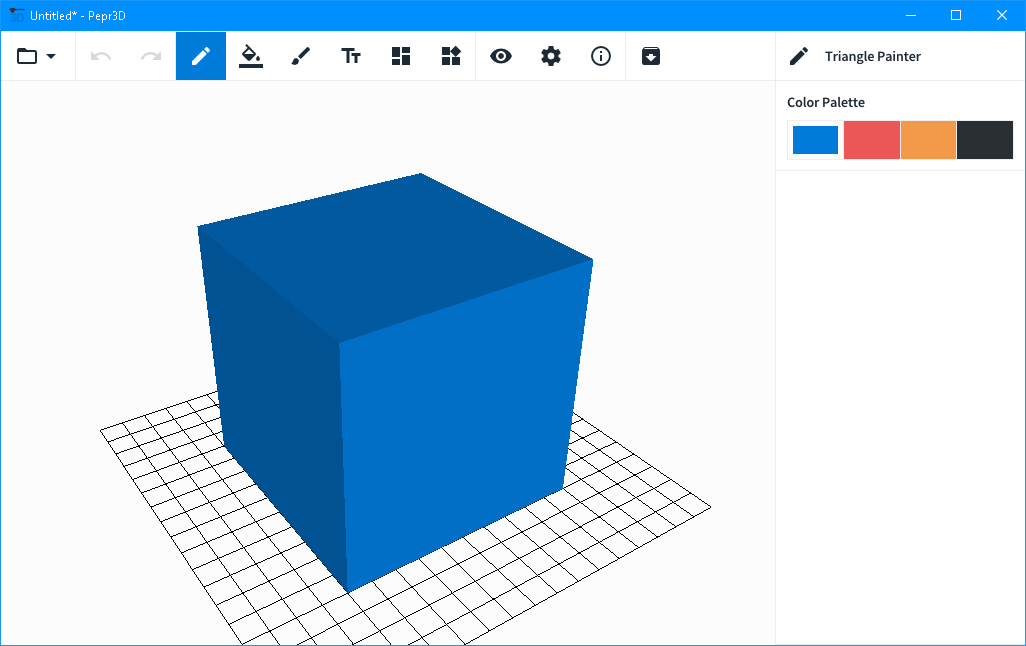
\includegraphics[scale=0.5]{images/pepr_cube.png}
	\caption{Pepr3D appearance after start-up.}
	\label{fig:pepr_cube}
\end{figure}

\subsection{Model manipulation}
You can manipulate the model by using your mouse. There are several ways to manipulate so you can reach and see any part of the model:

\begin{itemize}
\item \textbf{Rotation} -- Click and hold right mouse button and move.
\item \textbf{Translation} -- Press Ctrl + right mouse button and move, or press and hold the middle mouse button (mouse wheel) and move the mouse.
\item \textbf{Zoom} -- Scroll with the mouse wheel.
\end{itemize}

Left mouse button is dedicated to using selected tool.

\section{First model}
Now we can start working on a simple model with Pepr3D. First we have to acquire a 3D model, it should be in one of these file formats: \texttt{.stl}, \texttt{.ply}, \texttt{.obj}. The simplest way to acquire model is choose any model on the internet and download it. Or you can use any 3D modelling software and create one on your own. In this tutorial we use a simple low-polygon model of a Bulbasaur downloaded from Thingiverse\footnote{https://www.thingiverse.com/thing:327753}.

To import the model we can use a drag and drop gesture with the model file or we can browse for a model file after clicking \textit{Import} in the file menu.


\subsection{Painting the model}

After importing the model we can use any tool that our application provides to color the model as we want. In a few steps, we will show how to quickly color the imported model of our Bulbasaur with basic tools.

\begin{enumerate}
\item Select the \textit{Triangle Painter} tool, choose black color in the color palette.
\item Paint all triangles in each eye by clicking on them with the left mouse button. It is possible to click and drag to paint multiple adjacent triangles at once.
\item Use the same technique to paint its ears.

\begin{center}
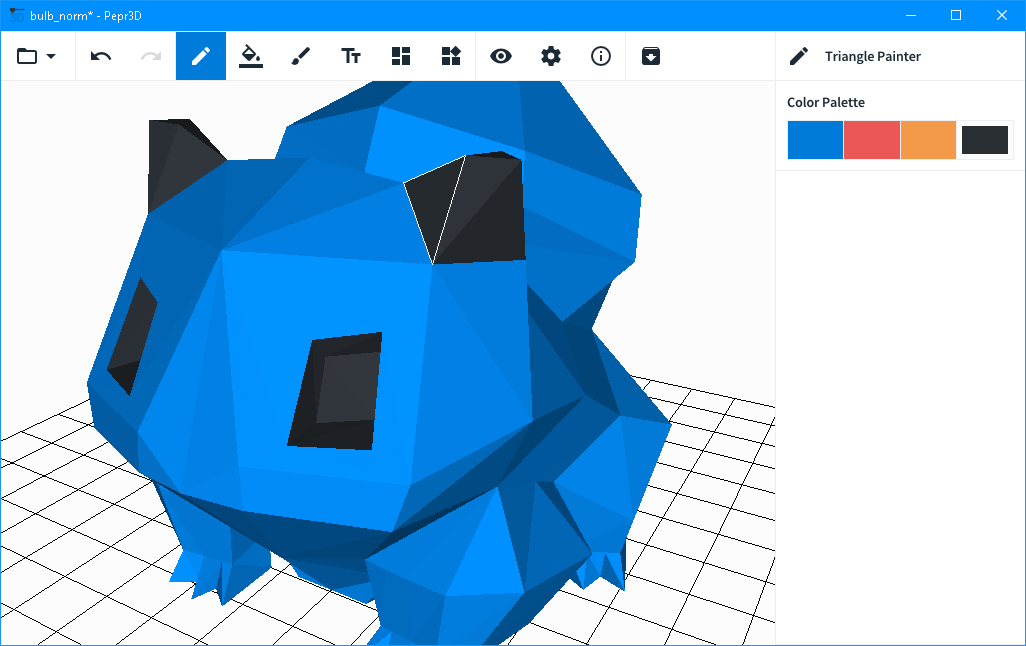
\includegraphics[scale=0.4]{images/bulb_eyes.png}
\end{center}

\item Choose another color (red) and select the \textit{Paint Bucket} tool.
\item Check \textit{Stop on sharp edges} in the side pane and set the \textit{Maximum angle} to 45$^\circ$.
\item Use the \textit{Paint Bucket} on any triangle on the "onion" on the back of the Bulbasaur. Click two more times on any unpainted triangle to paint the whole "onion" with red color.
\item Select the \textit{Triangle Painter} and the first color (blue) and recolor two triangles near the neck which have been painted extra by the \textit{Paint Bucket} in the previous step.

\begin{center}
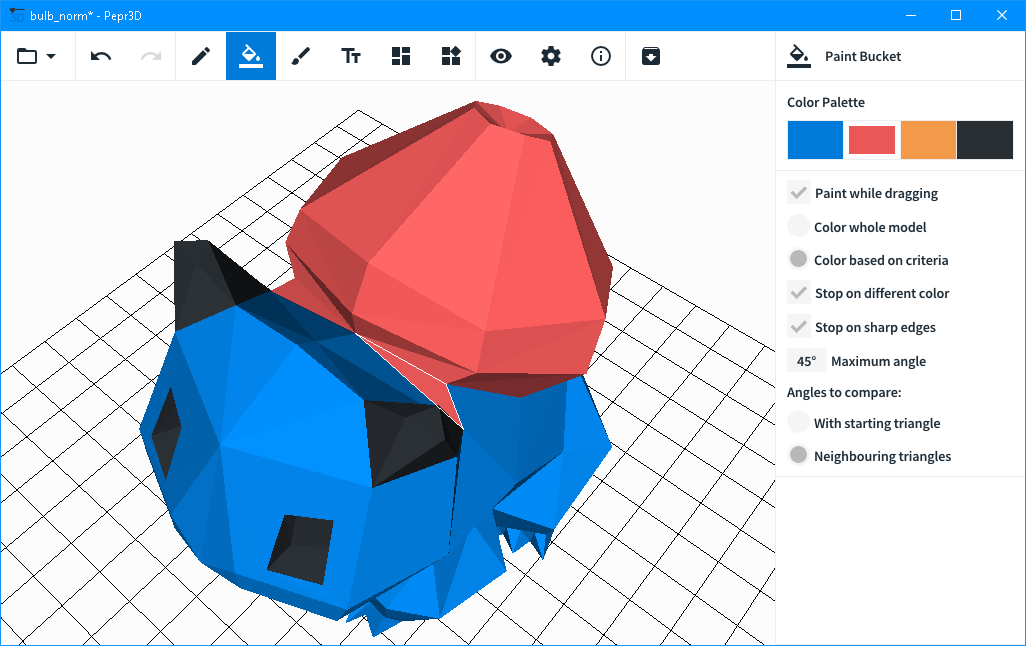
\includegraphics[scale=0.4]{images/bulb_onion.png}
\end{center}

\item Select the \textit{Brush} tool and check both the \textit{Respect original triangles} checkbox and the \textit{Paint outer ring} checkbox in the settings of the tool.
\item Set the brush size to about 4.0.
\item Choose orange and paint each leg. Do not forget to paint the legs from below.

\begin{center}
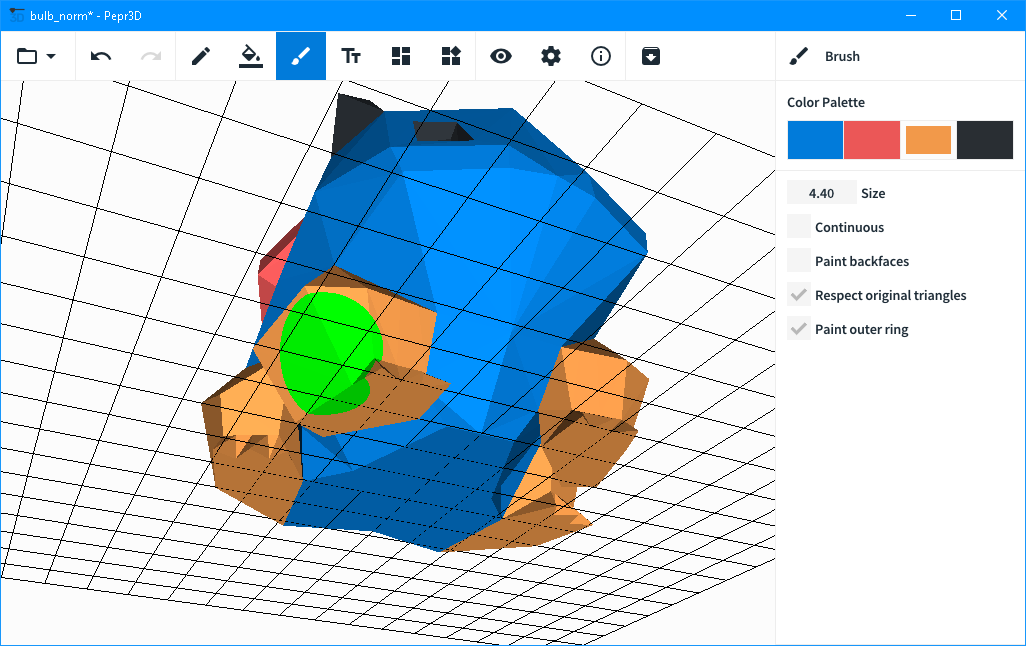
\includegraphics[scale=0.4]{images/bulb_legs.png}
\end{center}

\end{enumerate}


You can undo any step you did with any tool. For example, if you paint on a incorrect triangle, you can press \textit{Undo} (left arrow) in the toolbar to revert the mistake.

\subsection{Exporting the model}
Now the model is painted and we can proceed to model exporting. Before exporting the model itself we need to set the depth of color extrusion into the model. Exporting can be summarized in the following steps:


\begin{enumerate}
\item Open the \textit{Export Assistant} on the toolbar or click \textit{Export} in the file menu.
\item Click the \textit{Update extrusion preview!} button.
\item Lower the percentage of \textit{Max Preview height} to see into the model and see the thickness of model walls -- the extrusion depth.
\item Adjust the percentage of \textit{Depth} for the desired extrusion depth.
\item Update the preview by clicking on the \textit{Update extrusion preview!} button.
\item Repeat adjusting the depth and updating the preview until you are satisfied.
\item Click on \textit{Export files} and complete the export.
\end{enumerate}

\begin{figure}
	\centering
	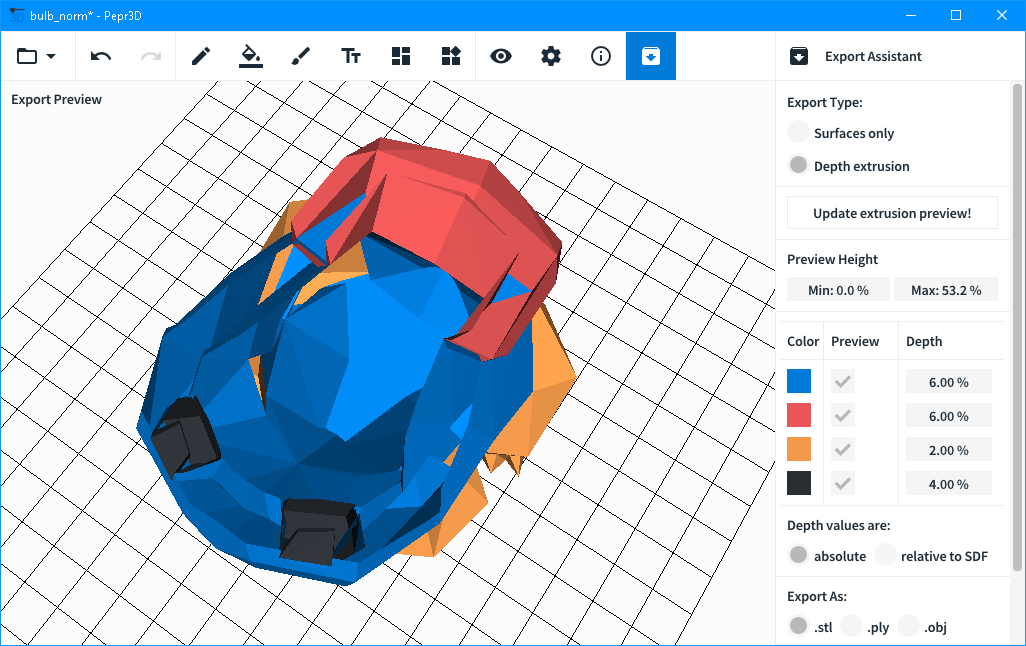
\includegraphics[scale=0.5]{images/bulb_export.png}
	\caption{Example of \textit{Export Assistant} with colored model.}
	\label{fig:bulb_export}
\end{figure}


Exported files can be now imported into any supported slicer and printed on a multimaterial 3D printer.




